% 图 74.10 —— 由 `checks/emit_hand.py` 自动拼出（probe 精测 + prims2 图元分解）
%%
% ⚠ 这是**稿子不是成品**：跑 `checks/checkhand.py 74.10` 看指标 + 看叠合图。
%%
%% ⚠ 待核：
%   · 本图 probe 报出阴影族 3 个 —— **本脚本不生成阴影**（要照原书手写）；prims2 的 strokes 里可能含阴影线，核对时留意别画重
%   · 可疑字形 1 项（空心圈 ⊙ 常被认成字母 o）—— 见文件末
%%
\documentclass[12pt]{standalone}
\usepackage{fontspec}
\setsansfont{Arial}
\newfontfamily\mfallback{DejaVu Sans}
\usepackage{tikz}
\usetikzlibrary{arrows.meta}
\begin{document}
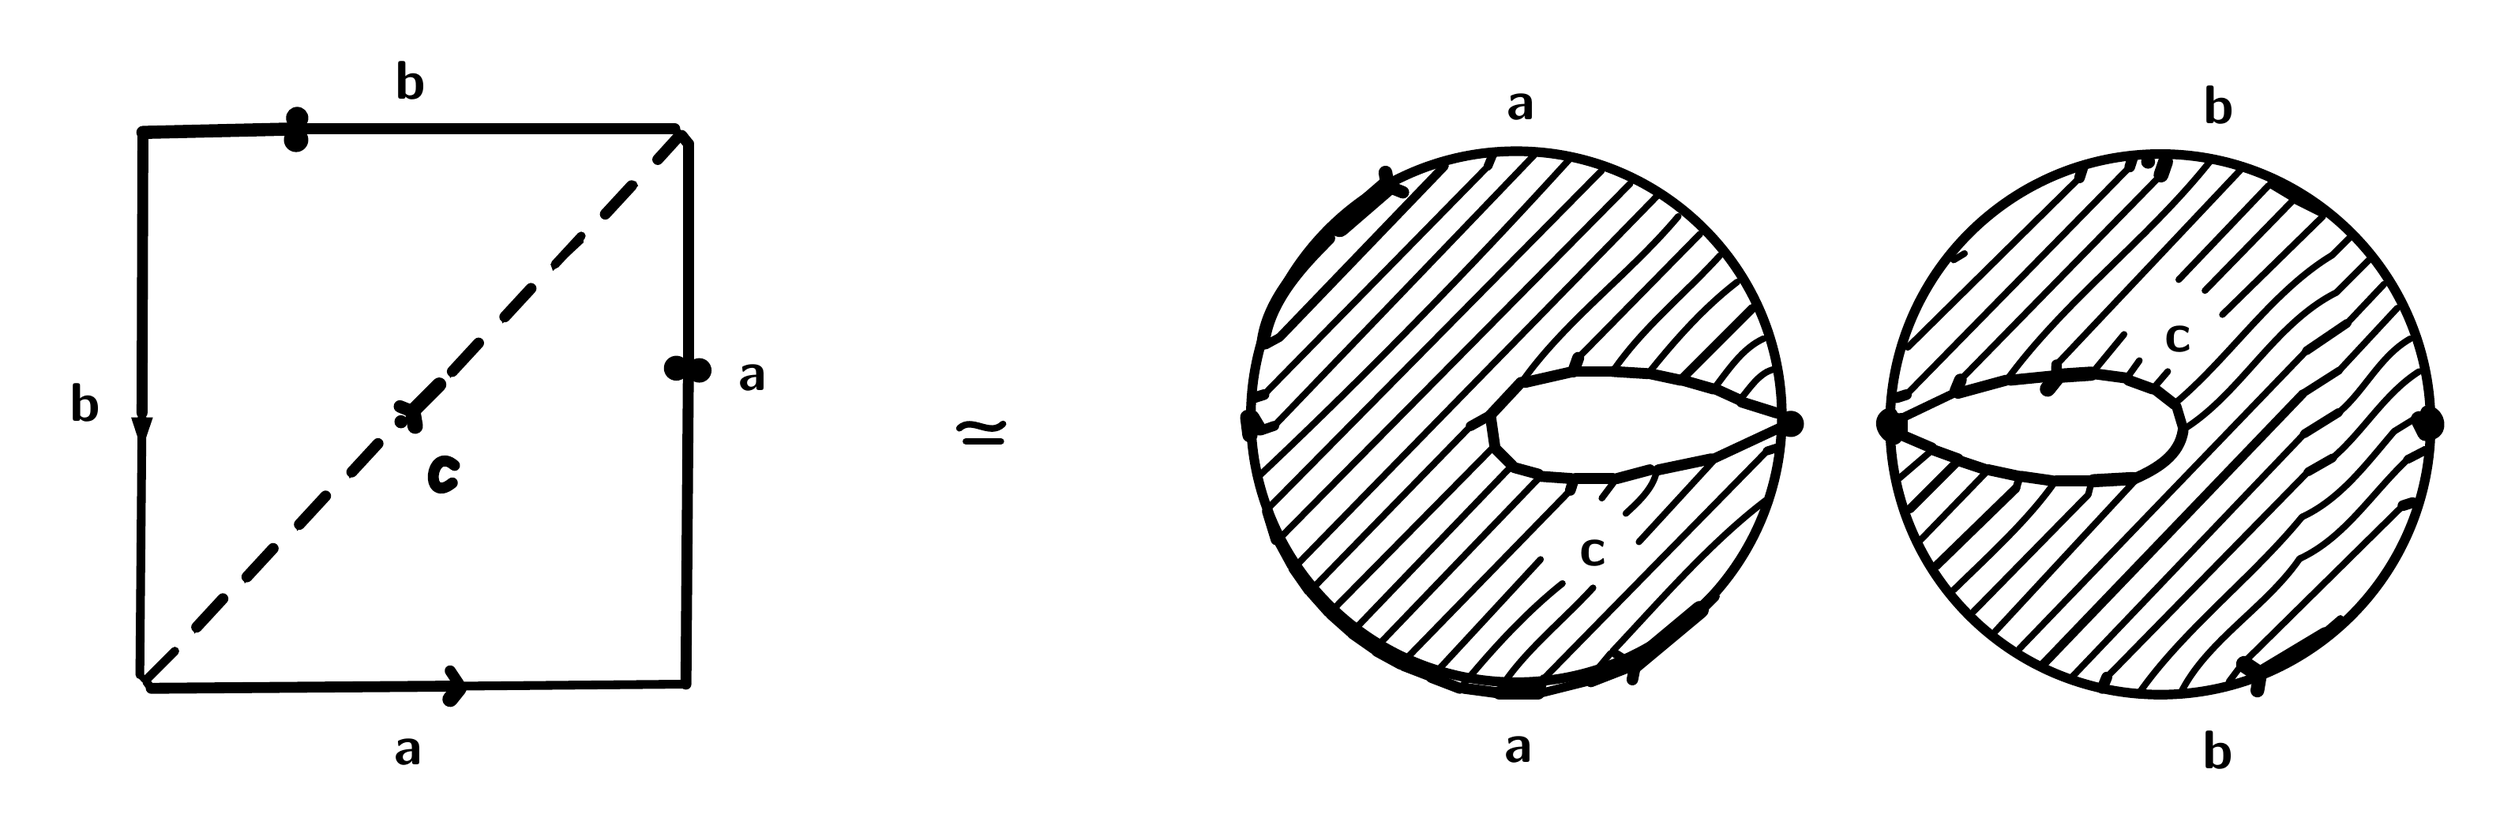
\begin{tikzpicture}[x=1pt, y=-1pt, line width=4.4pt, line cap=round, line join=round]

  %% ════ 填充区（prims2 的 fills）════
  \fill (281.0,73.0) -- (278.0,73.0) -- (268.0,84.0) -- (266.0,90.0) -- (268.0,90.0) -- (282.0,75.0) -- cycle;
  \fill (257.0,97.0) -- (255.0,97.0) -- (242.0,111.0) -- (243.0,114.0) -- (257.0,101.0) -- cycle;
  \fill (234.0,121.0) -- (232.0,121.0) -- (219.0,135.0) -- (220.0,138.0) -- (235.0,123.0) -- cycle;
  \fill (210.0,146.0) -- (208.0,146.0) -- (195.0,160.0) -- (196.0,163.0) -- (211.0,148.0) -- cycle;
  \fill (164.0,192.0) -- (162.0,192.0) -- (149.0,206.0) -- (150.0,209.0) -- (165.0,194.0) -- cycle;
  \fill (140.0,216.0) -- (138.0,216.0) -- (125.0,230.0) -- (126.0,233.0) -- (141.0,218.0) -- cycle;
  \fill (116.0,240.0) -- (114.0,240.0) -- (101.0,254.0) -- (102.0,257.0) -- (117.0,242.0) -- cycle;
  \fill (93.0,263.0) -- (91.0,263.0) -- (78.0,277.0) -- (79.0,280.0) -- (94.0,265.0) -- cycle;

  %% ════ 直线段（prims2 的 strokes）════
  \draw[line width=5.0pt] (305.0,162.0) -- (303.9,303.1);
  \draw[line width=4.0pt] (303.9,303.1) -- (201.0,304.0);
  \draw[line width=3.0pt] (693.0,60.0) -- (573.1,184.9);
  \draw[line width=4.5pt] (573.1,184.9) -- (567.0,187.0);
  \draw[line width=6.0pt] (126.0,49.0) -- (55.4,50.6);
  \draw[line width=5.0pt] (55.4,50.6) -- (55.0,179.0);
  \draw[line width=5.0pt] (759.0,164.0) -- (745.0,161.0);
  \draw[line width=3.0pt] (583.0,249.0) -- (748.0,80.0);
  \draw[line width=7.1pt] (180.0,185.0) -- (179.0,179.0);
  \draw[line width=5.0pt] (744.0,161.0) -- (728.0,160.0);
  \draw[line width=7.1pt] (200.0,305.0) -- (196.0,310.0);
  \draw[line width=5.0pt] (914.0,208.0) -- (900.0,205.0);
  \draw[line width=3.0pt] (1061.0,273.0) -- (1054.0,279.0);
  \draw[line width=6.3pt] (1024.0,300.0) -- (1023.0,306.0);
  \draw[line width=5.0pt] (682.0,203.0) -- (674.0,195.0);
  \draw[line width=5.0pt] (899.0,205.0) -- (887.0,201.0);
  \draw[line width=5.0pt] (302.0,52.0) -- (305.0,55.8);
  \draw[line width=5.0pt] (305.0,55.8) -- (305.0,159.0);
  \draw[line width=8.0pt] (738.0,294.0) -- (768.0,269.0);
  \draw[line width=5.0pt] (683.0,204.0) -- (694.0,207.0);
  \draw[line width=3.0pt] (869.0,237.0) -- (899.0,206.0);
  \draw[line width=4.9pt] (943.0,67.0) -- (941.6,71.4);
  \draw[line width=3.0pt] (941.6,71.4) -- (863.0,149.0);
  \draw[line width=4.0pt] (256.0,98.0) -- (244.0,111.0);
  \draw[line width=3.0pt] (893.0,270.0) -- (945.6,216.4);
  \draw[line width=3.0pt] (945.6,216.4) -- (947.0,211.0);
  \draw[line width=6.0pt] (860.0,188.0) -- (860.0,182.0);
  \draw[line width=3.4pt] (856.0,180.0) -- (859.0,181.0);
  \draw[line width=5.3pt] (737.0,301.0) -- (738.0,296.0);
  \draw[line width=5.7pt] (627.0,76.0) -- (632.0,78.0);
  % （略）线段 (56.0,180.0)-(61.0,177.0) 线宽6.1 —— 是箭头头那一坨，已由箭头头代替
  \draw[line width=3.0pt] (448.0,192.0) -- (432.0,192.0);
  \draw[line width=5.0pt] (975.0,168.0) -- (964.0,164.0);
  \draw[line width=3.0pt] (301.0,51.0) -- (298.8,49.0);
  \draw[line width=5.0pt] (298.8,49.0) -- (128.0,49.0);
  \draw[line width=6.3pt] (624.0,69.0) -- (625.0,75.0);
  \draw[line width=5.0pt] (686.0,165.0) -- (672.0,180.0);
  \draw[line width=3.0pt] (964.0,162.0) -- (969.0,155.0);
  \draw[line width=5.0pt] (886.0,170.0) -- (908.0,164.0);
  \draw[line width=3.0pt] (1074.0,109.0) -- (1059.1,123.9);
  \draw[line width=5.5pt] (710.0,160.0) -- (712.2,153.8);
  \draw[line width=3.0pt] (712.2,153.8) -- (768.0,97.0);
  \draw[line width=5.0pt] (710.0,160.0) -- (688.0,165.0);
  \draw[line width=5.0pt] (710.0,160.0) -- (728.0,160.0);
  \draw[line width=3.0pt] (967.0,210.0) -- (903.0,279.0);
  \draw[line width=5.0pt] (745.0,205.0) -- (730.0,209.0);
  \draw[line width=5.0pt] (103.0,254.0) -- (115.0,241.0);
  \draw[line width=3.0pt] (987.0,118.0) -- (1028.0,75.0);
  \draw[line width=6.5pt] (932.0,162.0) -- (947.0,161.0);
  \draw[line width=4.9pt] (966.0,62.0) -- (964.6,66.4);
  \draw[line width=3.0pt] (964.6,66.4) -- (862.4,170.6);
  \draw[line width=4.9pt] (862.4,170.6) -- (858.0,172.0);
  \draw[line width=6.0pt] (1054.0,280.0) -- (1024.0,298.0);
  \draw[line width=4.5pt] (774.0,200.0) -- (804.0,186.0);
  \draw[line width=5.0pt] (749.0,205.0) -- (773.0,200.0);
  \draw[line width=3.0pt] (859.0,209.0) -- (873.0,197.0);
  \draw[line width=4.0pt] (57.0,301.0) -- (70.0,288.0);
  \draw[line width=4.0pt] (729.0,289.0) -- (737.0,294.0);
  \draw[line width=5.0pt] (197.0,160.0) -- (209.0,147.0);
  \draw[line width=3.0pt] (884.0,109.0) -- (889.0,106.0);
  \draw[line width=6.0pt] (948.0,210.0) -- (966.0,209.0);
  \draw[line width=5.0pt] (151.0,206.0) -- (163.0,193.0);
  \draw[line width=5.0pt] (127.0,230.0) -- (139.0,217.0);
  \draw[line width=3.0pt] (599.0,270.0) -- (673.0,195.0);
  \draw[line width=5.0pt] (948.0,161.0) -- (963.0,163.0);
  \draw[line width=9.0pt] (625.0,75.0) -- (603.0,94.0);
  \draw[line width=3.8pt] (1100.0,179.0) -- (1097.0,181.0);
  \draw[line width=5.0pt] (660.0,305.0) -- (675.0,307.0);
  \draw[line width=3.0pt] (717.0,301.0) -- (727.0,289.0);
  \draw[line width=4.0pt] (886.0,201.0) -- (864.0,223.0);
  \draw[line width=3.0pt] (1053.0,89.0) -- (1007.0,134.0);
  \draw[line width=4.0pt] (768.0,268.0) -- (774.0,262.0);
  \draw[line width=5.0pt] (728.0,209.0) -- (711.0,209.0);
  \draw[line width=5.0pt] (952.0,305.0) -- (954.1,299.9);
  \draw[line width=3.0pt] (954.1,299.9) -- (1046.1,206.0);
  \draw[line width=4.0pt] (1046.1,206.0) -- (1057.5,199.5);
  \draw[line width=5.0pt] (803.0,179.0) -- (787.0,174.0);
  \draw[line width=4.0pt] (1091.7,200.3) -- (1100.0,196.0);
  \draw[line width=5.0pt] (200.0,303.0) -- (196.0,297.0);
  \draw[line width=4.0pt] (1060.3,178.7) -- (1044.4,188.6);
  \draw[line width=3.0pt] (1044.4,188.6) -- (938.0,300.0);
  \draw[line width=4.0pt] (632.0,295.0) -- (645.0,300.0);
  \draw[line width=5.0pt] (80.0,277.0) -- (92.0,264.0);
  \draw[line width=4.0pt] (884.0,170.0) -- (861.0,181.0);
  \draw[line width=5.0pt] (929.0,210.0) -- (915.0,208.0);
  \draw[line width=5.0pt] (631.0,294.0) -- (620.0,288.0);
  \draw[line width=3.0pt] (1016.0,67.0) -- (931.1,156.9);
  \draw[line width=4.8pt] (931.1,156.9) -- (931.0,161.0);
  \draw[line width=5.0pt] (709.0,209.0) -- (695.0,208.0);
  \draw[line width=4.0pt] (651.0,66.0) -- (575.6,144.4);
  \draw[line width=4.0pt] (575.6,144.4) -- (569.0,148.0);
  \draw[line width=5.0pt] (619.0,287.0) -- (609.0,280.0);
  \draw[line width=7.1pt] (927.0,168.0) -- (931.0,163.0);
  \draw[line width=5.0pt] (674.0,194.0) -- (672.0,180.0);
  \draw[line width=3.0pt] (1085.6,187.4) -- (1096.0,181.0);
  \draw[line width=5.0pt] (774.0,168.0) -- (760.0,164.0);
  \draw[line width=7.6pt] (1017.0,294.0) -- (1023.0,298.0);
  \draw[line width=5.0pt] (860.0,189.0) -- (874.0,195.0);
  \draw[line width=3.0pt] (740.0,238.0) -- (774.0,201.0);
  \draw[line width=3.0pt] (570.0,223.0) -- (723.0,68.0);
  \draw[line width=5.0pt] (658.0,305.0) -- (645.0,300.0);
  \draw[line width=3.0pt] (1065.0,99.0) -- (1057.2,106.8);
  \draw[line width=6.0pt] (676.0,307.0) -- (694.0,307.0);
  \draw[line width=3.0pt] (976.0,167.0) -- (982.0,160.0);
  \draw[line width=3.0pt] (1016.0,294.0) -- (1010.0,302.0);
  \draw[line width=4.9pt] (1094.0,220.0) -- (1089.6,221.4);
  \draw[line width=3.0pt] (1089.6,221.4) -- (1017.0,293.0);
  \draw[line width=3.5pt] (914.0,209.0) -- (912.6,213.4);
  \draw[line width=4.0pt] (912.6,213.4) -- (876.0,249.0);
  \draw[line width=3.0pt] (694.0,209.0) -- (620.0,286.0);
  \draw[line width=3.0pt] (729.0,210.0) -- (723.0,218.0);
  \draw[line width=3.0pt] (999.0,123.0) -- (1039.0,82.0);
  \draw[line width=3.0pt] (609.0,279.0) -- (681.0,204.0);
  \draw[line width=5.0pt] (301.0,52.0) -- (291.0,63.0);
  \draw[line width=6.6pt] (566.0,186.0) -- (563.0,181.0);
  \draw[line width=7.0pt] (562.0,189.0) -- (561.0,181.0);
  \draw[line width=5.0pt] (910.0,164.0) -- (930.0,162.0);
  \draw[line width=5.0pt] (718.0,302.0) -- (736.0,295.0);
  \draw[line width=3.0pt] (645.0,300.0) -- (695.0,246.0);
  \draw[line width=4.0pt] (581.0,249.0) -- (575.0,238.0);
  \draw[line width=3.0pt] (590.0,260.0) -- (663.0,185.0);
  \draw[line width=4.5pt] (663.0,185.0) -- (672.0,180.0);
  \draw[line width=4.0pt] (55.0,181.0) -- (54.0,298.8);
  \fill (50.0,181.0) -- (60.0,181.0) -- (54.9,196.0) -- cycle;
  \draw[line width=3.0pt] (54.0,298.8) -- (56.0,301.0);
  \draw[line width=3.0pt] (632.0,293.0) -- (708.6,214.4);
  \draw[line width=4.9pt] (708.6,214.4) -- (710.0,210.0);
  \draw[line width=4.0pt] (769.0,269.0) -- (775.0,263.0);
  \draw[line width=3.0pt] (575.0,237.0) -- (736.0,74.0);
  \draw[line width=3.8pt] (57.0,302.0) -- (59.2,305.0);
  \draw[line width=5.0pt] (59.2,305.0) -- (199.0,304.0);
  \draw[line width=3.0pt] (1087.0,131.0) -- (1060.5,159.5);
  \draw[line width=3.5pt] (1060.5,159.5) -- (1043.9,170.1);
  \draw[line width=4.0pt] (1043.9,170.1) -- (925.0,294.0);
  \draw[line width=5.0pt] (1053.0,87.0) -- (1041.0,81.0);
  \draw[line width=5.0pt] (279.0,75.0) -- (267.0,88.0);
  \draw[line width=3.0pt] (962.0,143.0) -- (948.0,160.0);
  \draw[line width=5.0pt] (589.0,260.0) -- (582.0,250.0);
  \draw[line width=4.0pt] (760.0,163.0) -- (792.0,131.0);
  \draw[line width=7.7pt] (1100.0,188.0) -- (1097.0,182.0);
  \draw[line width=5.0pt] (233.0,122.0) -- (221.0,135.0);
  \draw[line width=5.0pt] (574.0,237.0) -- (570.0,224.0);
  \draw[line width=3.0pt] (1081.0,120.0) -- (1064.1,137.9);
  \draw[line width=4.0pt] (1064.1,137.9) -- (1045.4,150.6);
  \draw[line width=3.0pt] (1045.4,150.6) -- (914.0,287.0);
  \draw[line width=5.0pt] (598.0,270.0) -- (590.0,261.0);
  \draw[line width=5.7pt] (173.0,176.0) -- (178.0,178.0);
  \draw[line width=5.0pt] (599.0,271.0) -- (608.0,279.0);
  \draw[line width=5.0pt] (985.0,175.0) -- (976.0,168.0);
  \draw[line width=5.0pt] (786.0,173.0) -- (775.0,168.0);
  \draw[line width=4.5pt] (986.0,176.0) -- (989.0,186.0);
  \draw[line width=4.0pt] (695.0,306.0) -- (696.4,300.6);
  \draw[line width=3.0pt] (696.4,300.6) -- (798.6,196.4);
  \draw[line width=4.0pt] (798.6,196.4) -- (803.0,195.0);
  \draw[line width=5.0pt] (946.0,210.0) -- (931.0,210.0);
  \draw[line width=4.9pt] (564.0,172.0) -- (568.4,170.6);
  \draw[line width=3.0pt] (568.4,170.6) -- (670.9,66.1);
  \draw[line width=4.0pt] (670.9,66.1) -- (673.0,61.0);
  \draw[line width=6.8pt] (981.0,64.0) -- (978.9,70.1);
  \draw[line width=3.0pt] (978.9,70.1) -- (887.1,163.9);
  \draw[line width=5.8pt] (887.1,163.9) -- (885.0,169.0);
  \draw[line width=5.0pt] (1030.0,74.0) -- (1040.0,80.0);
  \draw[line width=5.0pt] (875.0,196.0) -- (886.0,200.0);
  \draw[line width=6.5pt] (179.0,178.0) -- (191.0,166.0);
  \draw[line width=4.0pt] (696.0,307.0) -- (716.0,302.0);

  %% ════ 曲线（prims2 的 curves —— 三段式，坐标同为 (y,x)）════
  \draw[line width=5.0pt] (197.0,211.0) .. controls (183.9,221.6) and (186.6,193.2) .. (198.0,203.0);
  \draw[line width=3.0pt] (802.0,159.0) .. controls (795.6,160.1) and (791.0,167.2) .. (787.0,172.0);
  \draw[line width=3.0pt] (449.0,184.0) .. controls (442.8,190.1) and (434.9,180.4) .. (429.0,186.0);
  \draw[line width=5.0pt] (989.0,187.0) .. controls (987.4,198.5) and (976.8,204.6) .. (967.0,209.0);
  \draw[line width=7.0pt] (1102.0,188.0) .. controls (1107.0,187.2) and (1105.4,179.8) .. (1101.0,179.0);
  \draw[line width=3.0pt] (1059.1,123.9) .. controls (1031.2,137.9) and (1015.6,169.7) .. (990.0,186.0);
  \draw[line width=3.0pt] (728.0,160.0) .. controls (741.5,140.2) and (760.9,124.7) .. (777.0,107.0);
  \draw[line width=3.0pt] (1057.5,199.5) .. controls (1071.7,187.3) and (1081.2,170.0) .. (1097.0,160.0);
  \draw[line width=3.0pt] (728.0,288.0) .. controls (750.0,264.6) and (772.9,238.1) .. (798.0,219.0);
  \draw[line width=3.0pt] (988.0,307.0) .. controls (999.8,283.3) and (1027.2,267.7) .. (1042.3,245.7);
  \draw[line width=3.0pt] (1042.3,245.7) .. controls (1062.8,236.3) and (1075.4,215.7) .. (1091.7,200.3);
  \draw[line width=3.0pt] (1093.0,145.0) .. controls (1079.1,152.8) and (1071.9,169.1) .. (1060.3,178.7);
  \draw[line width=3.0pt] (969.0,307.0) .. controls (989.1,278.3) and (1020.8,254.2) .. (1043.4,226.6);
  \draw[line width=3.0pt] (1043.4,226.6) .. controls (1061.0,218.5) and (1073.1,202.0) .. (1085.6,187.4);
  \draw[line width=3.0pt] (884.0,260.0) .. controls (899.4,244.9) and (917.8,228.3) .. (930.0,211.0);
  \draw[line width=3.0pt] (687.0,164.0) .. controls (706.5,136.7) and (736.1,115.1) .. (758.0,89.0);
  \draw[line width=3.0pt] (1057.2,106.8) .. controls (1030.2,123.0) and (1010.4,153.4) .. (986.0,174.0);
  \draw[line width=7.0pt] (855.0,180.0) .. controls (849.3,181.8) and (852.6,188.8) .. (857.0,190.0);
  \draw[line width=3.0pt] (566.0,208.0) .. controls (615.2,161.6) and (663.0,112.6) .. (709.0,62.0);
  \draw[line width=3.0pt] (909.0,163.0) .. controls (935.7,126.9) and (974.1,98.4) .. (1002.0,63.0);
  \draw[line width=3.0pt] (745.0,160.0) .. controls (756.8,145.3) and (770.0,130.5) .. (785.0,119.0);
  \draw[line width=3.0pt] (705.0,257.0) .. controls (688.3,270.3) and (673.0,287.0) .. (659.0,304.0);
  \draw[line width=3.0pt] (719.0,259.0) .. controls (704.6,274.7) and (686.5,288.9) .. (676.0,306.0);
  \draw[line width=3.0pt] (775.0,167.0) .. controls (781.3,158.7) and (787.8,149.1) .. (797.0,145.0);
  \draw[line width=3.0pt] (734.0,225.0) .. controls (739.4,220.0) and (746.4,213.7) .. (748.0,206.0);
  \draw[line width=6.0pt] (598.0,99.0) .. controls (584.7,112.2) and (570.3,128.0) .. (568.0,147.0);

  %% ════ 圆 / 椭圆（probe 精测）════
  \draw (978.6,184.2) circle (123.7);
  \draw (683.9,180.7) circle (121.5);

  %% ════ 实心点 ════
  \fill (126.0,44.0) circle (5.1);
  \fill (125.5,54.0) circle (5.6);
  \fill (973.0,64.0) circle (3.2);
  \fill (299.5,158.5) circle (5.7);
  \fill (310.0,159.5) circle (5.6);
  \fill (809.5,184.0) circle (6.0);
  \fill (173.5,183.0) circle (3.0);

  %% ════ 标签（probe 直接给的 \node 行）════
  %% ⚠ 全部补了 fill=white：文字在最上层，否则与曲线交叉干扰
     \node[anchor=center,inner sep=0pt,fill=white,font=\fontsize{30.7}{38.3}\selectfont] at (177.8,26.8) {\textsf{\textbf{\textit{b}}}};   % box(168,14,17,23)
     \node[anchor=center,inner sep=0pt,fill=white,font=\fontsize{31.6}{39.5}\selectfont] at (1005.3,37.8) {\textsf{\textbf{\textit{b}}}};   % box(995,25,18,23)
     \node[anchor=center,inner sep=0pt,fill=white,font=\fontsize{32.0}{40.0}\selectfont] at (686.1,39.1) {\textsf{\textbf{\textit{a}}}};   % box(677,29,16,17)
     \node[anchor=center,inner sep=0pt,fill=white,font=\fontsize{31.4}{39.3}\selectfont] at (986.8,145.1) {\textsf{\textbf{\textit{c}}}};   % box(978,135,16,17)
     \node[anchor=center,inner sep=0pt,fill=white,font=\fontsize{33.0}{41.2}\selectfont] at (334.6,163.1) {\textsf{\textbf{\textit{a}}}};   % box(325,153,17,17)
     \node[anchor=center,inner sep=0pt,fill=white,font=\fontsize{30.0}{37.5}\selectfont] at (28.8,174.2) {\textsf{\textbf{\textit{b}}}};   % box(19,162,17,22)
     \node[anchor=center,inner sep=0pt,fill=white,font=\fontsize{31.4}{39.3}\selectfont] at (718.8,243.1) {\textsf{\textbf{\textit{c}}}};   % box(710,233,16,17)
     \node[anchor=center,inner sep=0pt,fill=white,font=\fontsize{30.0}{37.5}\selectfont] at (1004.8,333.2) {\textsf{\textbf{\textit{b}}}};   % box(995,321,17,22)
     \node[anchor=center,inner sep=0pt,fill=white,font=\fontsize{32.0}{40.0}\selectfont] at (685.1,333.1) {\textsf{\textbf{\textit{a}}}};   % box(676,323,16,17)
     \node[anchor=center,inner sep=0pt,fill=white,font=\fontsize{32.0}{40.0}\selectfont] at (177.1,334.1) {\textsf{\textbf{\textit{a}}}};   % box(168,324,16,17)

  % 钉死画布：否则超出的图元/控制点会把页面撑大，1:1 回比就失准
  \pgfresetboundingbox
  \path[use as bounding box] (0,0) rectangle (1124,354);
\end{tikzpicture}
\end{document}

% ⚠ 待核清单（probe 拿不准，人眼过一遍）：
%   · 未识别/跳过：⑤ 跳过/未识别的字形
